\documentclass[../template]{subfiles}

\begin{document}
\section{Flusso a costo minimo}
\begin{center}
    \begin{tikzpicture}[rotate=90, EdgeStyle/.style={->}]
        \Vertices[unit = 2]{circle} {1, 2, 3, 4, 5}
        \Edge[label=$5/9$](1)(2)
        \Edge[label=$15/4$](1)(4)
        \Edge[label=$2/3$](1)(3)
        \Edge[label=$3/11$](2)(4)
        \Edge[label=$2/4$](3)(4)
        ;
    \end{tikzpicture}
\end{center}
\subsection{Classificazione dei nodi}
Nei problemi di flusso a costo minimo, i nodi sono divisi in tre categorie, in base a $b_i$:
\begin{enumerate}
    \item Nodi sorgente: $b_i > 0$, in essi viene realizzato il prodotto.
    \item Nodi di transito: $b_i = 0$, il prodotto transita, senza variazioni
    \item Nodi destinazione: $b_i < 0$, dove il prodotto viene consumato.
\end{enumerate}
La proprietà $\sum_i^n b_i = 0$, quando non risulta valida, è forzabile aggiungendo un fittizio
con $b_{n+1} = -\sum_i^n b_i$, collegato a tutti i nodi sorgente, attraverso archi di costo 0 e capacità $+\infty$.

\subsubsection{Nel caso di archi con capacità illimitata}
\begin{wrapfigure}{r}{.33\textwidth}
    \centering
    \begin{tikzpicture}[rotate=90, EdgeStyle/.style={->}]
        \Vertices[unit=2]{circle}{1, 2, 3, 4, 5}
        \Edge[label=$5$](1)(2)
        \Edge[label=$-2$](1)(3)
        \Edge[label=$2$](1)(5)
        \Edge[label=$-4$](2)(3)
        \Edge[label=$0$](3)(4)
        \Edge[label=$6$](4)(2)
        \Edge[label=$3$](4)(5)
        \Edge[label=$4$](5)(3)
        ;
        \node[draw] at ([shift={(0:.7cm)}]1)   {$b=2$};
        \node[draw] at ([shift={(0:.7cm)}]2)   {$b=5$};
        \node[draw] at ([shift={(180:.7cm)}]3) {$b=5$};
        \node[draw] at ([shift={(180:.7cm)}]4) {$b=5$};
        \node[draw] at ([shift={(0:.7cm)}]5)   {$b=5$};
    \end{tikzpicture}
    \caption{$b_i$ sono indicati vicino al nodo}
    \label{graph:infty_flux}
\end{wrapfigure}
Prendiamo come esempio la rete $G = (V, A)$ in figura \ref{graph:infty_flux}.


\end{document}
